%
% fig-homotopie.tex
%
% (c) 2025 Prof Dr Andreas Müller
%
\begin{figure}
\centering
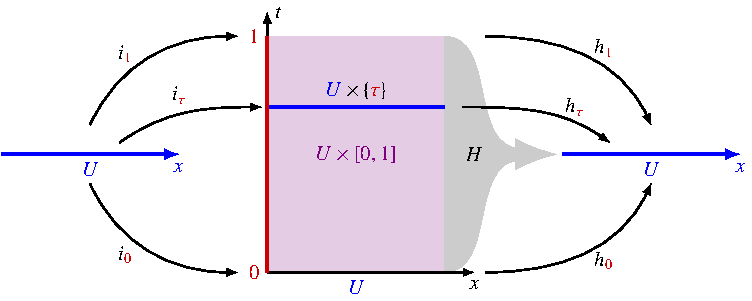
\includegraphics{chapters/060-pformen/images/homotopie.pdf}
\caption{Eine Homotopie $H$ ist eine Abbildung $U\times[0,1]$, die
die Abbildung $h_0\colon U\to U$ in die Abbildung $h_1\colon U\to U$
deformiert.
Die Abbildung $h_{\tau}$ entsteht durch Einsetzen des Wertes $\tau$
in das zweite Argument von $H$, was gleichbedeutend ist mit der
Zusammensetzung von $H$ mit $i_\tau$: $h_\tau=H\circ i_\tau$.
\label{buch:pformen:fig:homotopie}}
\end{figure}
